\documentclass{beamer}
\usetheme{metropolis}
\usepackage{graphicx}
\usepackage{amsmath}
\usepackage{makecell}
\title{A History of Science in Latin America (INTD290): Unit 1.2}
\author{Jordan Hanson}
\institute{Whittier College Department of Physics and Astronomy}

\begin{document}
\maketitle

\section{Outline}

\begin{frame}{Outline}
\textit{Comparitive medical treatments - chapter 1 content.} \\
\alert{Chapter 2 content}
\begin{enumerate}
\item Mining and agriculture in Nueva Espa\~{n}a
\item Construction of scientific communities
\item The formation of scientific literature and community, importation of scientific texts
\item Catholic religious orders in Latin America
\item Galileo, Kepler, and the Heliocentric system of the world
\end{enumerate}
\alert{Activities}
\begin{enumerate}
\item Timelines of discoveries and development
\item Geographical illustrations with Google Earth
\item Digital Storytelling on cosmic rays and the solar wind
\end{enumerate}
\end{frame}

\section{More on Literary Societies and Journals}

\begin{frame}{More on Literary Societies and Journals}
\small
\begin{figure}
\centering
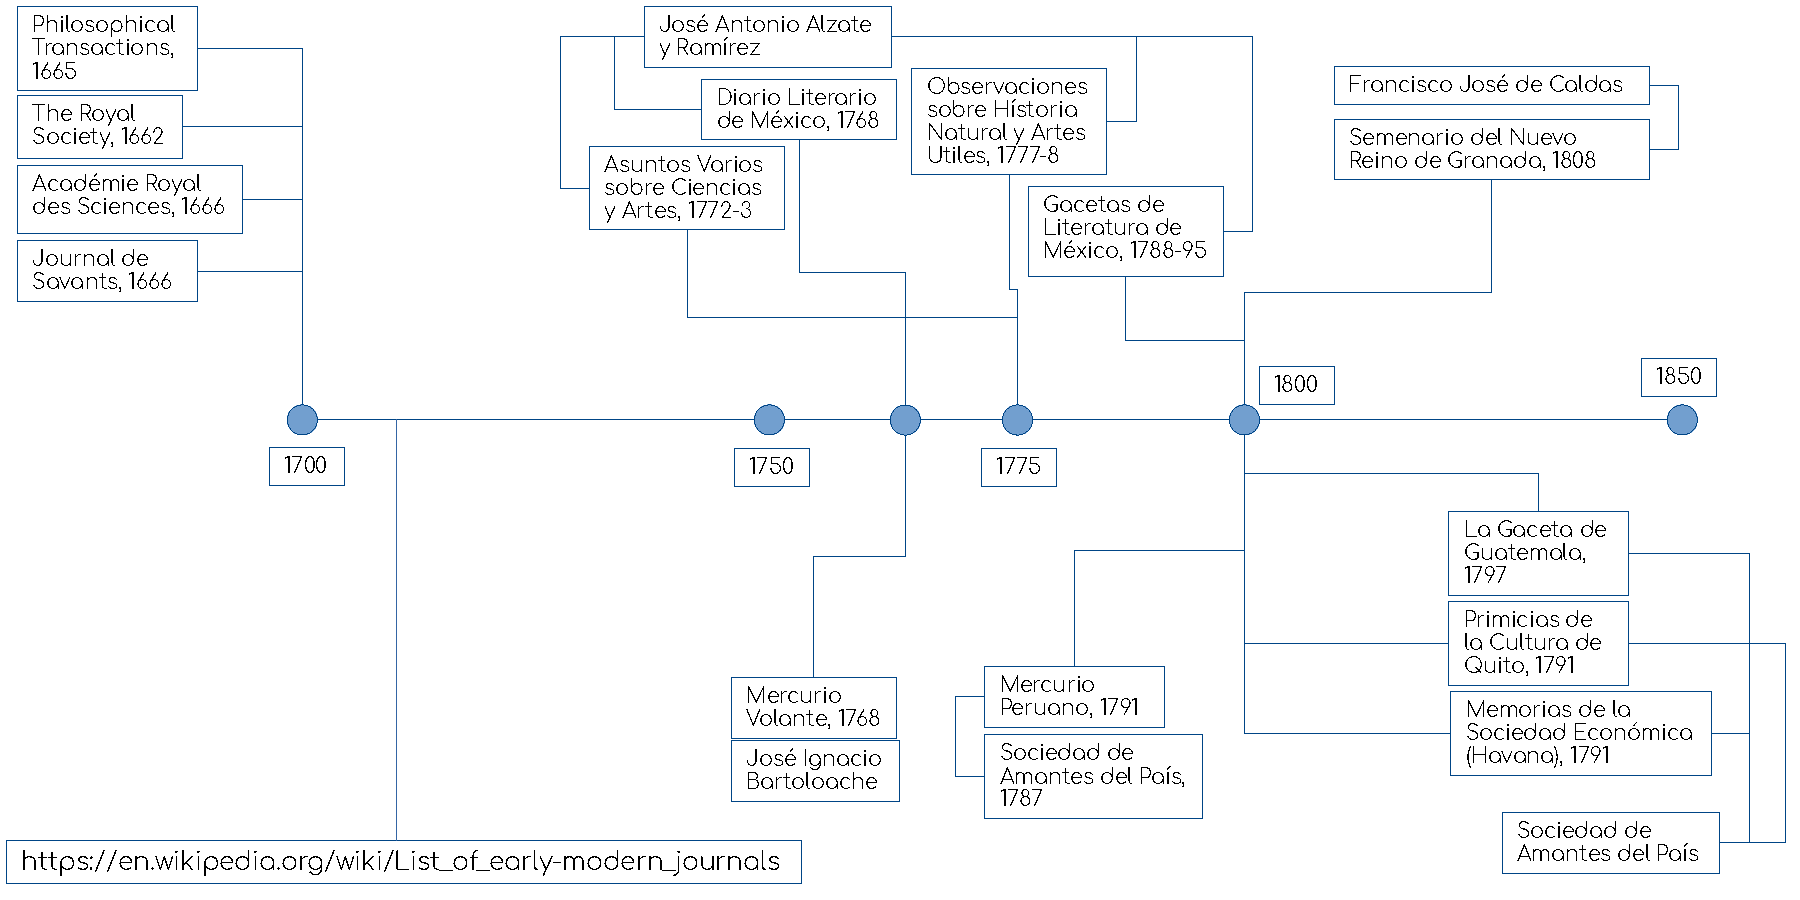
\includegraphics[width=0.95\textwidth]{figures/TimeLine1.pdf}
\caption{\label{fig:time1} A visualization of scientific journals of the 18th Century Latin American society.  Note the prevalance of Societies of Friends of the Country, versus Royal Societies.  Note also the gap between 1700-1750.  For a complete list of journals in the gap, see the link at lower left.}
\end{figure}
\end{frame}

\begin{frame}{More on Literary Societies and Journals}
\small
\begin{enumerate}
\item Friends of the Country versus Royal Society
\item Alzate, Bartolache (Mexico)
\item Other journals notg shown: \textit{Gacetas de Caracas, 1808}, \textit{Semenario de Agricultura, Industria y Comercio, Buenos Aires, 1802}, \textit{O Patriota, 1813-1814}
\item Mining processes debated in these journals, the patio process versus the Born process
\begin{itemize}
\item Fausto de Elh\'{u}yar (Spain), Baron von Nordenflicht (Sweden)
\item Jos\'{e} Antonio Alzate (New Spain) wrote in \textit{Observaciones} in 1787 that \'{A}lvaro Alonso Barba discovered the ``Born method'' in 1640.  The Creoles noted that the Born method was not as efficient in this situation.
\end{itemize}
\end{enumerate}
\end{frame}

\section{Colleges and Curricula}

\begin{frame}{Colleges and Curricula}

\end{frame}

\end{document}